\documentclass{article} % For LaTeX2e
\usepackage{nips11submit_e,times,amsmath,amsfonts, graphicx, subfigure,amssymb}
%\documentstyle[nips10submit_09,times,art10]{article} % For LaTeX 2.09


\title{Unlabeled graph classification}


\author{
Joshua T.~Vogelstein\thanks{ Use footnote for providing further information
about author (webpage, alternative address)---\emph{not} for acknowledging
funding agencies.} \\
Department of Applied Mathematics and Statistics\\
Johns Hopkins University\\
Baltimore, MD 21218 \\
\texttt{joshuav@jhu.edu} \\
\And
John M.~Conroy \\
Affiliation \\
Address \\
\texttt{conroyjohnm@gmail.com} \\
\AND
Steven Kratzer \\
Affiliation \\
Address \\
\texttt{sgkratz@gmail.com} \\
\AND
Lou \\
Affiliation \\
Address \\
\texttt{conroyjohnm@gmail.com} \\
\AND
Glen A.~Coppersmith \\
Affiliation \\
Address \\
\texttt{coppersmith@jhu.edu} \\
\And
Mark Dredze \\
Affiliation \\
Address \\
\texttt{mdredze@cs.jhu.edu} \\
\And
R.~Jacob Vogelstein \\
Affiliation \\
Address \\
\texttt{Jacob.Vogelstein@jhuapl.edu} \\
\And
Carey E.~Priebe \\
Affiliation \\
Address \\
\texttt{cep@jhu.edu} \\
}


\newcommand{\fix}{\marginpar{FIX}}
\newcommand{\new}{\marginpar{NEW}}

\newcommand{\jv}{Joshua Vogelstein}
\newcommand{\jhu}{Johns Hopkins University}
%\newcommand{\hp}{https://jshare.johnshopkins.edu/jvogels3/public_html/}
\newcommand{\ema}{joshuav@jhu.edu}

\newcommand{\eqdef}{\overset{\triangle}{=}}
\newcommand{\D}[2]{\frac{\partial #1}{\partial #2}}
\newcommand{\DD}[2]{\frac{\partial ^2 #1}{\partial #2 ^2}}
\newcommand{\DDD}[3]{\frac{\partial ^2 #1}{\partial #2 \partial #3}}
\newcommand{\Di}[2]{\frac{\partial ^i #1}{\partial #2 ^i}}
\newcommand{\grad}{\nabla}
\newcommand{\Hess}{\nabla\nabla}

\providecommand{\ve}[1]{\boldsymbol{#1}}
\providecommand{\norm}[1]{\left \lVert#1 \right  \rVert}
\providecommand{\deter}[1]{\lvert #1 \rvert}
\providecommand{\abs}[1]{\left \lvert #1 \right \rvert}
\newcommand{\argmax}{\operatornamewithlimits{argmax}}
\newcommand{\argmin}{\operatornamewithlimits{argmin}}
\newcommand{\T}{^{\ensuremath{\mathsf{T}}}}           % transpose
\newcommand{\EE}{\mathbb{E}}           % expected value
\newcommand{\PP}{\mathbb{P}}           % probability
\newcommand{\II}{\mathbb{I}}           % indicator function
\newcommand{\QQ}{\mathbb{Q}}           
\newcommand{\SSS}{\mathbb{S}}           

\newcommand{\bth}{\ve{\theta}}
\newcommand{\bTh}{\ve{\Theta}}
\newcommand{\hbth}{\widehat{\thet}}

\providecommand{\mc}[1]{\mathcal{#1}}
\providecommand{\mb}[1]{\boldsymbol{#1}}
\providecommand{\mbb}[1]{\mathbb{#1}}
\providecommand{\mv}[1]{\vec{#1}}
\providecommand{\mh}[1]{\hat{#1}}
\providecommand{\mt}[1]{\widetilde{#1}}
\providecommand{\mhc}[1]{\hat{\mathcal{#1}}}
\providecommand{\mhb}[1]{\hat{\boldsymbol{#1}}}
\providecommand{\mvb}[1]{\vec{\boldsymbol{#1}}}
\providecommand{\mtb}[1]{\widetilde{\boldsymbol{#1}}}

\newcommand{\Real}{\mathbb{R}}
\newcommand{\conv}{\rightarrow}
\newcommand{\iid}{\overset{iid}{\sim}}
\newcommand{\defeq}{\overset{\triangle}{=}}

\newcommand{\mcE}{\mathcal{E}}
\newcommand{\mcT}{\mathcal{T}}
\newcommand{\mcG}{\mathcal{G}}
\newcommand{\mcM}{\mathcal{M}}
\newcommand{\mcL}{\mathcal{L}}
\newcommand{\hatmcE}{\widehat{\mcE}}
\newcommand{\hatp}{\widehat{p}}
\newcommand{\hatP}{\widehat{P}}
\newcommand{\hatQ}{\widehat{Q}}
\newcommand{\hatL}{\widehat{L}}
\newcommand{\mhP}{\widehat{\PP}}
\newcommand{\tildeA}{\widetilde{A}}
\newcommand{\GG}{\mathbb{G}}
\newcommand{\qap}{\texttt{QAP} }
\newcommand{\qapa}{\texttt{QAP}$_1$ }
\newcommand{\qapn}{\texttt{QAP$_n$} }
\newcommand{\qapb}{\texttt{QAP$_{100}$} }


%\nipsfinalcopy % Uncomment for camera-ready version

\begin{document}

 
\maketitle

\begin{abstract}
Because graphs can encode more information in their structure than vectors, they are becoming increasingly popular data structures for representing information.  While the last century has witnessed the development of a plethora of statistical tools for the analysis of data, the vast majority of these tools natively operate in vector spaces, not graph spaces.  Thus, algorithms for even relatively simple statistical inference tasks, such as two-class classification,  are essentially absent for graph data.  In this work, we propose a number of complementary algorithms to classify graphs, with special attention to the possibility of unknown vertex labels.  Since exactly solving the graph-matching problem is currently computational intractable, we consider several approximate approaches.  We introduce a multiple-restart Frank-Wolfe approach to solving the graph matching problem by formulating it as a quadratic assignment problem.  Although this approach has superior performance than previous state-of-the-art approaches to the graph matching problem, even when it ``should'' do well in classification problems, it is outperformed by a graph invariant strategy.  This is just the beginning. 
\end{abstract}

\section{Introduction}


The statistical analysis of collections of graphs is becoming an increasingly popular desideratum \cite{Bunke2011}.  Specifically, we consider the following idealized and simplified scenario. Let $\GG: \Omega \mapsto \mc{G}$ be a graph-valued random variable taking values $G\in \mc{G}$. Each graph is a 4-tuple: $G=(\mc{V},\mc{E},\mc{L},\mc{A})$, where $\mc{V}$ is a set of $|\mc{V}|=n_V$ vertices, $\mc{E}$ is a set of $|\mc{E}|=E$ edges, $\mc{L}=\{1,\ldots,n_V\}=[n_V]$ is a set of vertex labels (one per vertex), and $\mc{A}$ is a set of edge attributes.  Elements of $\mc{A}$ could be binary matrices (for unweighted graphs) or higher-order tensors (for mult-graphs).  Let $Y$ be a Bernoulli random variable, $Y: \Omega \mapsto \{0,1\}$, such that each graph has an associated class.  Given a collection of graphs and classes,  we assume they were jointly sampled independently and identically from some true but unknown distribution, $\{(\GG_i,Y_i)\}_{i \in [n]} \iid F_{\GG,Y}(\cdot; \theta)$.  Note that $F_{\GG,Y}(\cdot; \bth)$ is but one of a (possibly infinite) set of distributions, collectively comprising the model: $\mc{F_{\GG,Y}}=\{F_{\GG,Y}(\cdot; \bth) : \theta \in \bTh\}$, where $\bTh$ is the set of feasible parameters.  The goal of such an analysis is to learn about the relationship between $\GG$ and $Y$.   Standard classification techniques fail in this domain as they typically require classifying objects that live in finite dimensional Euclidean space, whereas the object of interest here are graphs (even finite ones do not natively live in Euclidean space).  In this work, therefore, we propose novel extensions of several classification algorithms appropriate for the graph domain.



\section{Graph Classification} % (fold)
\label{sec:graph_classification}


The graph classification problem may be stated thusly: given training data $\mc{T}_n=\{(\GG_i,Y_i)\}_{i \in [n]}$, and a new graph, $\GG$, estimate the new graph's corresponding class, $Y$, assuming each graph/class pair was sampled identically and independently from some true but unknown distribution, $\mc{T}_n,(\GG,Y) \iid F_{\GG,Y}(\cdot; \theta)$ .  Given an appropriately defined loss-function, such as misclassification rate: $L_h=\PP[h(\GG) \neq Y]$, one can then search for the function $h^* \in \mc{H}$ that minimizes the loss function of interest:
\begin{align}
	h^* = \argmin_{h \in \mc{H}} \PP[h(\GG) \neq Y].
\end{align}
In general, $h^*$ is unavailable and dependent on the model, $\mc{F}_{\GG,Y}$ (which includes the vertex labels).  When $h^*$ is unavailable, one can utilize training data, $\mc{T}_n$, to obtain $\mh{h}$, an approximation to $h^*$:
\begin{align}
	\mh{h} \approx \argmin_{h \in \mc{H}} \PP[h(\GG) \neq Y | \mc{T}_n],
\end{align}
where $\approx$ indicates that in general, we will not be able to find the actual minimum in the set $\mc{H}$. Regardless, any approach necessarily estimates a decision boundary in the space of graphs separating them into two classes.  %We consider a few distinct such approaches to constructing such a decision boundary:

% \subsection{Graph dissimilarity based approach approach} % (fold)
% \label{sub:_k__n_nearest_neighbor_approach}

% \subsection{Graph dissimilarity based approach approach} % (fold)
% \label{sub:_k__n_nearest_neighbor_approach}


% % section graph_classification (end)
% \section{Unlabeled sticky wicket}

In certain graph classification problems the vertex labels are unknown.  In other words, instead of observing $(\mc{V},\mc{E},\mc{L},\mc{A})$ for each graph, we only observe the triple, $(\mc{V},\mc{E},\mc{A})$, which we refer to as an \emph{unlabeled graph}.  In such scenarios, one is essentially faced with a graph isomorphism problem, which can be approached in at least two ways.  First, one could try to \emph{graph match}, that is, find a common set of labels for the vertices of the graphs, so that the graphs have the same adjacency matrix. Second, one can project the graphs into a quotient space that is invariant to the labels.  This can be a negative check for isomorphisms: if a set of graphs have different representations in the quotient space, then they are not isomorphic to one another.  We consider both approaches as possible subroutines as part of a classification function.




% \section{Methods} % (fold)
% \label{sec:methods}

\subsection{Graph Matching} % (fold)
\label{sec:quadratic_assignment_problem}

A graph can be represented by its adjacency matrix, $A$, assuming the edge attributes are univariate.  Unlabeled graphs, on the other hand, can be represented by a set of adjacency matrices, $\{QAQ\T : Q \in \mc{Q}\}$, where $Q$ is any permutation matrix.  Given a pair of unlabeled graphs, determining whether they are isomorphic with respect to one another is equivalent to determining whether one can find an adjacency matrix of one graph that is identical to the other's.  This problem can be cast as a \emph{quadratic assignment problem} (QAP):
 \begin{align} \label{eq:QAP}
	Q_{QAP} \defeq Q_{QAP}(A,B)= \argmin_{Q \in \mc{Q}} \norm{Q A Q\T - B}^2_F,
\end{align}
where $A$ and $B$ are adjacency matrix representations of two different graphs. A bit of linear algebra simplifies Eq. \eqref{eq:QAP}: % \cite{Horn1990}, and demonstrates that the above objective function 
%shows that Eq \eqref{eq:QAP} can be simplified:
\begin{align} \label{eq:qap}
	\argmin_{Q \in \mc{Q}} \norm{Q A Q\T - B}^2_F = \argmin_{Q \in \mc{Q}} - tr(B\T QAQ\T) - tr(QAQ\T B),			
\end{align}
which is equivalent to the standard representation of the quadratic assignment problem \cite{Conte2004}:
\begin{align}
	\mh{\sigma}= \argmin_{\sigma} a_{\sigma(i), \sigma(j)} b_{ij} = \argmin_{q \in \mc{Q}} q_{ij} a_{ij}, q_{ji} b_{ij}
\end{align}
where $\sigma$ is a permutation function, that is, $\sigma: [n] \mapsto [n]$.  Unfortunately, Eq. \eqref{eq:QAP} is an NP-complete problem \cite{Garey1979a}. The primary difficulty in solving Eq. \eqref{eq:QAP} is the discrete non-convex constraint set.  Thus, it is natural to consider an approximation with the constraints relaxed.  Since the convex hull of permutation matrices is the set of doubly stochastic matrices, we define the approximate quadratic assignment problem:
\begin{align} \label{eq:tqap}
	Q_{AQAP} \defeq Q_{AQAP}(A,B) = \argmin_{Q \in \mc{D}} \norm{Q A Q\T - B}^2_F,
\end{align}
where $\mc{D}$ is the set of doubly stochastic matrices.  When the permutation matrix constraint is relaxed, the equivalence relation shown in Eq. \eqref{eq:qap} no longer holds.  Nonetheless, we proceed by attempting to solve:
\begin{align} \label{eq:nqap}
	\mh{Q}_{AQAP} \approx \argmin_{Q \in \mc{D}} - tr(B\T QAQ\T) - tr(QAQ\T B),
\end{align}
considering it an auxiliary function for which we can compute gradients and ascend a likelihood, unlike the permutation constrained case.  

The Frank-Wolfe (FW) algorithm is a successive linear programming algorithm for nonlinear programming problems; specifically, for quadratic problems with linear (equality and/or inequality) constraints. Let $f(Q)=- tr(B\T QAQ\T) - tr(QAQ\T B)$.  With each iteration $j$, the FW algorithm takes the following steps:

\paragraph{Step 1: Compute the gradient} % (fold)
\label{par:step_1_computing_the_gradient}

The gradient of $f$ with respect to $Q$ is given by:
\begin{align} \label{eq:grad}
	\nabla_Q^{(j)} = \partial f / \partial Q^{(j)} =  A Q^{(j)} B\T + A\T Q^{(j)} B.
\end{align}

% paragraph step_1_computing_the_gradient (end)

\paragraph{Step 2: Find the closest doubly stochastic matrix} % (fold)
\label{par:step_2_finding_the_closest_doubly_stochastic_matrix}

Instead of directly descending this gradient, we search for the direction of the doubly stochastic matrix closest to this gradient. Noting that that direction may be computed by the dot-product operator, we have:
\begin{align}\label{eq:dir}
	W^{(j)} = \argmin_{W^{(j)} \in \mc{D}} \langle \nabla_Q^{(j)},W^{(j)} \rangle. %  \sum_{i,j=1}^m 	\left( 	\nabla_Q^{(j)}\circ W^{(j)} \right)_{ij}.
\end{align}
Eq. \eqref{eq:dir} can be solved as a Linear Assignment Problem (LAP).  More specifically, a LAP can be written as:
\begin{align} \label{eq:LAP}
	Q_{\text{LAP}} \defeq Q_{\text{LAP}}(A,B) = \argmin_{Q \in \mc{Q}} \norm{QA - B }^2_F,
\end{align}
which, when $B=I$, can be simplified:
\begin{align} \label{eq:proja}
	Q_{\text{LAP}}(A,I) \argmin_{Q \in \mc{Q}} \norm{QA - I}_F^2 &= \argmin_{Q \in \mc{Q}} (QA-I)\T (QA-I) 
\nonumber\\ &=\argmin_{Q \in \mc{Q}} A\T Q\T QA -2QA - II = \argmin_{Q \in \mc{Q}}  -\langle Q, A \rangle.  
\end{align}
In other words, letting $B=I$, the projection of a matrix onto its nearest doubly stochastic matrix is a LAP problem.  While Eq. \eqref{eq:proja} cannot be solved directly, as above, we can relax the permutation matrix constraint to the doubly stochastic matrix constraint:
\begin{align}\label{eq:relaxed}
	Q_{\text{LAP}}(A,I) = \argmin_{Q\in\mc{D}} -\langle Q, A \rangle. 
\end{align}
Since the permutation matrices are the vertices of the set of doubly stochastic matrices, finding the minimum of Eq. \eqref{eq:relaxed} is guaranteed to yield a permutation matrix (as minima are necessarily at the vertices).  Thus, letting $A=\nabla_Q^{(j)}$, solving Eq. \eqref{eq:relaxed}---which is a linear problem with linear and non-negative constraints---is equivalent to solving Eq. \eqref{eq:dir}.  Fortunately, the Hungarian algorithm solves any LAP in $\mc{O}(n^3)$ \cite{Burkard2009}, thus this projection is relatively efficient.\footnote{More efficient algorithms are available for certain special cases, that is, whenever the matrix-vector multiplication operation is fast (for example, when both $A$ and $B$ are sparse).}
% paragraph step_2_finding_the_closest_doubly_stochastic_matrix (end)

\paragraph{Step 3: Update the direction} % (fold)
\label{par:step_3_updating_the_direction}


Given $W^{(j)}$, the new direction is given by:
\begin{align}
	d^{(j)}=W^{(j)}-Q^{(j)}.
\end{align}

% paragraph step_3_updating_the_direction (end)

\paragraph{Step 4: Line search} % (fold)
\label{par:step_4_line_search}


Given this direction, one can then perform a line search to find the doubly stochastic matrix that minimizes the objective function along that direction:
\begin{align}
	\alpha^{(j)} = \argmin_{\alpha \in [0,1]} f(Q^{(j)} + \alpha^{(j)} d^{(j)}).
\end{align}
This can be performed exactly, because $f$ is a quadratic function.  

% paragraph step_4_line_search (end)

\paragraph{Step 5: Update $Q$} % (fold)
\label{par:step_5_update_q_}

Finally, the new estimated doubly stochastic matrix is given by:
\begin{align}\label{eq:update}
	Q^{(j+1)} = Q^{(j)} + \alpha^{(j)} d^{(j)}.
\end{align}

% paragraph step_5_update_q_ (end)

\paragraph{The grand finale} % (fold)
\label{par:the_final_iteration}

Steps 1--5 are iterated until convergence, computational budget limits, or some other stopping criterion is met.  These 5 steps collective comprise the FW algorithm.  Note that while $Q^{(j)}$ will generally not be a permutation matrix, we do not project $Q^{(j)}$ back onto the set of permutation matrices between each iteration, as that projection requires $\mc{O}(n^3)$ time. After the final iteration, however, we have $\mh{Q}_{AQAP}$, which we project onto the set of permutation matrices:
\begin{align} \label{eq:proj}
	\mh{Q}_{QAP} = \argmin_{Q \in \mc{Q}} \langle \mh{Q}_{AQAP}, Q \rangle,
\end{align}
which is a LAP, and yields approximate solution to QAP.  Let \qap indicate this algorithm: FW appended with a projection onto the permutation matrices.

% paragraph the_final_iteration (end)

\paragraph{Multiple restarts} % (fold)
\label{par:putting_it_all_together}


Note that \qap will not generally achieve the global optimum even of Eq. \eqref{eq:tqap}, because $f$ is not necessarily positive definite.  This is clear upon computing the Hessian of $f$  with respect to $Q$:
\begin{align}
	\nabla_Q^2  =  B \otimes A + B\T \otimes A\T,
\end{align}
where $\otimes$ indicates the Kronecker product. This means that the initialization, $Q^{(0)}$, will be important.  While any doubly stochastic matrix would be a feasible initial point, two choices seem natural: (i) the ``flat doubly  stochastic matrix,'' $J=\ve{1}\T \ve{1}/n_V$, which is the middle of the feasible region, and (ii) the identity matrix, which is a permutation matrix.  Therefore, if we run the FW algorithm once, we always start with one of those two.  If we use multiple restarts, each initial point is ``near'' the flat matrix.  Specifically, we sample $J'$, a random doubly stochastic matrix using 10 iterations of Sinkhorn balancing \cite{Sinkhorn1964}, and let $Q^{(0)}=(J+J')/2$.  We refer to multiple re-starts of \qap with subscripts, that is, the performance of \qapn is the best result of $n$ pseudo-random re-starts of \texttt{QAP}.  Note that \qap natively operates on matrices, which could correspond to either weighted or unweighted graphs.

% paragraph putting_it_all_together (end)


\subsection{Graph Invariants} % (fold)
\label{sub:graph_invariants}

A graph invariant (GI) is any function that maps a graph to a scalar whose value is independent of the vertex labels, $T: (\mc{V},\mc{E},\mc{A}) \mapsto \Real$ (note that often graph invariants are defined to operate only on unweighted graphs, that is, $T: (\mc{V},\mc{E}) \mapsto \Real$).  By defining a set of GIs, one can embed a collection of graphs into a quotient space invariant to vertex labels.  Whenever this quotient space is a subset of finite dimensional Euclidean space, all standard machine learning classifiers may be implemented to solve the classification problem.  

% subsection graph_invariants (end)


\section{Unlabeled Graph Classification Algorithms} % (fold)
\label{sec:algorithms}

Below we provide an example, and briefly discuss, three complementary approaches to solving unlabeled graph classification problems.  Each strategy uses one of the two above approaches to dealing with the graph isomorphism problem as a subroutine.

\subsection{A graph dissimilarity approach: \texttt{$k$NN} $\circ$ \qap} % (fold)
\label{ssub:_k_nn_circ_qap}

Define a dissimilarity on graph spaces: $d: \mc{G} \times \mc{G} \mapsto \Real_+$, in which one can compute the dissimilarity between any pair of graphs. Given an adjacency matrix representation, many such dissimilarities are possible (e.g., graph edit distance, Hamming distance, etc.).  It is becoming increasingly popular to use a \emph{graph kernel}, $\kappa(G,G')=\langle \phi(G), \phi(G') \rangle$, where $\phi(\cdot): \mc{G} \mapsto \EE$, as the dissimilarity \cite{Bunke2011}.  Graph kernels have a number of desirable properties, perhaps most notably, that one can then use standard \emph{kernel machines} to classify \cite{Vapnik1998}.	Regardless, given any dissimilarity, one can apply at least two different kinds of classifiers.

% : nearest neighbor style classifiers and interpoint-dissimilarity based classifiers \cite{Duin2011}.  

First, one could implement a nearest neighbor style classifiers, such as the $k_n$ nearest neighbor ($k$NN) classifier.  In addition to being universally consistent\footnote{A sequence of $k$NN classifiers is guaranteed to converge to the Bayes optimal classifier  if  as $n \conv \infty$, $k \conv \infty$ but $k/n \conv 0$ \cite{Devroye1997}.}, $k$NN classifiers are computationally efficient, in that they only require $n+1$ graph dissimilarity computations (assuming a single test graph).  

Alternately, one could implement an interpoint-dissimilarity matrix based algorithm \cite{Duin2011}. This strategy has the advantage of using all available information to generate a class prediction, but a disadvantage that it requires $(n+1)^2$ graph dissimilarity computations. Moreover, it may be more sensitive to outliers.

For simplicity, we only consider the $k$NN strategy here.  Specifically, given a test adjacency matrix, $A$, find $\mh{Q}_i^A=\mh{Q}_{QAP}(A,B_i)$ for all $n$ training adjacency matrices, $\{B_i\}_{i \in [n]}$.  Given these solutions, let $\mt{A}_i=\mh{Q}_i^A A {\mh{Q}_i^A}{}\T$ for all $i$. Given a suitable dissimilarity $d: \mc{A} \times \mc{A} \mapsto \Real_+$, one can compute $d(\mt{A}_i,B_i)$ for all $i \in [n]$, and sort them: $d_{(1)} \leq d_{(2)} \leq \cdots \leq d_{(n)}$.  Let the $k_n$ nearest neighbors of $A$ be the graphs with the $k_n$ smallest distances, $\{d_{(1)},\ldots, d_{(j)}\}$.  The estimated class of the training sample $A$ is then the plurality class of the $k_n$ nearest neighbors: $\mh{y}=\argmax_{y} \II\{\sum_{i \in [k_n]} y_{(i)} = y \}$. Call this algorithm \texttt{$k$NN} $\circ$ \texttt{QAP}.

% subsubsection _k_nn_circ_qap (end)


\subsection{A graph model approach: \texttt{BPI}$\circ$\qap} % (fold)
\label{ssub:bayes_plugin_circ_qap}

First assume a model, $\mc{F}_{\GG,Y}$.  The model of graphs and classes may be factorized into (i) a class-conditional random graph model: $\mc{F}_{\GG  | Y} = \{F_{\GG|Y}[\cdot; \bth_Y] : \bth_Y \in \bTh\}$, and (ii) a class prior model, $\mc{F}_Y = \{F_Y[\cdot; \pi_Y] : \pi_Y \in (0,1)\}$.  Given such a factorization, one could then, for instance, estimate $\{\bth,\pi\}$ and then use standard model-based classifiers, such as the Bayes plugin (BPI) classifier.  

However, if all the training graphs are unlabeled, unless the class-conditional signal is independent of the vertex labels, one must somehow deal with the absent labels.  Sometimes a ``canonical'' labeling is somehow natural, and can be searched for.  Otherwise, one could \qap all the training graphs to the test graph.  This approach has the unfortunate consequence of making all the training graphs more similar to one another, disregarding the class labels.  Another option would be to select a ``prototype'' from each class. Although several prototype selection strategies have been studied, prototype selection is still problematic \cite{Bunke2011}.  Finally, one could generate prototype for each class, using all available information.  This approach is intriguing but complicated.  Each of these alternatives essentially defines a canonical labeling per class.

Regardless of how a canonical labeling is chosen per class, given this canonical labeling, a graph model approach takes the following steps.  First, align each graph in each class to its class prototype using \texttt{QAP}$_n$.  Second, estimate the likelihood parameters for each class, $\{\bth_Y\}_{Y \in \{0,1\}}$, as well as the class-priors. Third, the test graph can then be \texttt{QAP}ed to the prototype of each class.  Fourth, compute the posterior probability of the test graph coming from each class, by plugging in the parameters to the Bayes classifier.  Finally, let the estimated class be the \emph{maximum a posteriori} class.  Call this algorithm \texttt{BPI} $\circ$ \texttt{QAP}.


% subsubsection bayes_plugin_circ_qap (end)

% subsection graph_isomorphism_approach (end)

\subsection{A graph invariant approach: \texttt{CW}$\circ$\texttt{GI} } % (fold)
\label{sub:graph_invariant_approach}

To use graph invariants to classify, one first must choose as set of graph invariants.  Unfortunately, there is no known set of graph invariants that collectively solve the graph isomorphism problem \cite{Conte2004}.  Fortunately, some recent theoretical work shows that certain graph invariants have greater discriminability with regard to certain graph inference tasks \cite{Ruhkhin2011}. With that in mind, we generalize a standard set of unweighted graph invariants---described fully in \cite{CPP11}---developing their weighted graph invariant counterparts. We describe each briefly:
\begin{itemize}
	\item $T_{weight}$: total weight of all the edges in the graph
	\item $T_{maxweight}$, is the max over $d(v)$ for all $v \in \mc{V}$, where $d(v)$ is the sum of all weights incident to vertex $v$	
	\item $T_{MAW_g}$: a greedy approximation of the maximum average weight (MAW), akin to maximum average degree
	\item $T_{MAW_e}$: an eigenvalue approximation of MAW
	\item $T_{wS_1}$: the maximum weighted locality statistic, akin to the typical scan statistic, but sums the weight of edges in each neighborhood rather than just the number of edges.
	\item $T_{Dijkstra}$: the average Dijkstra path distance between each pair of vertices
	% \item $T_{size}$ is the number of edges in the graph.
	% \item $T_{maxdegree}$ is the $\max_v d(v)$ for all $v \in \mc{V}$, where $d(v)$ is the degree of vertex $v$.
	% \item $T_{MAD_g}$ is a greedy approximation of the maximum average degree.
	% \item $T_{MAD_e}$ is an eigenvalue approximation of the same.
	% \item $T_{S_1}$ is the maximum locality statistic, as described in \cite{Priebe}.
	% \item $T_{triangles}$ is the number of triangles (paths of length 3) in the graph.
	% \item $T_{cc}$ is the average clustering coefficient.
	% \item $T_{averagepathlength}$, $T_{closeness}$, and $T_{betweenness}$ are all measures of the path lengths required to traverse between arbitrary vertices or edges.
\end{itemize}

For each graph $G_i$ in the training set, we compute a graph invariant vector: $\mb{T}_i: \mc{G} \mapsto \Real^d$.  We stack these $n$ $d$-dimensional vectors to form a matrix $\mb{T} \in \Real^{n \times d}$.  Letting $T_{ij}$ indicate the $i^{th}$ graph invariant of the $j^{th}$ graph, and normalize each element to be between zero and one according to:  $T_{ij} \leftarrow \frac{T_{ij} - \min_i (T_{ij})}{\max_i(T_{ij}) - \min_i(T_{ij})}$.

% We then whiten this matrix to control for the divergence means and scales of the various graph invariants, $\mb{T} \rightarrow \mb{E}\mb{\Lambda}^{-1/2}\mb{E}\T \mb{T}$, where $\mb{E}\mb{\Lambda}\mb{E}\T$ is the eigenvalue decomposition of the covariance matrix,$\EE[\mb{T}\mb{T}\T]$ \cite{Hyvarinen2000}.  
Now, to estimate the class of a test graph, we first compute its invariant vector, $\mb{t}$, and normalize it appropriately.  We then apply a variety of machine learning algorithms, including $k$NN, linear classifiers, and SVMs.  For the below connectome data, the best performing algorithm is the exact confidence weighted classifier \cite{Crammer2008}.  Call this algorithm \texttt{CW}$\circ$\texttt{GI}.

% subsection graph_invariant_approach (end)

% section algorithms (end)


\section{Results}

\subsection{QAP benchmarks vs. PATH algorithm}

We first compare the performance of \qapn with recent state-of-the-art approaches on the QAP benchmark library \cite{Burkard1997}.  Specifically, \cite{Zaslavskiy2009} reported improved performance in all but two cases, in which the QPB method of Cremers et al. \cite{Schellewald2001} achieved a lower minimum.  We compare \qapn with the previous best performing algorithm.  In \emph{all} cases, \texttt{QAP}$_3$ outperforms the previous best result, often by orders of magnitude in terms of relative error. In three cases, \qapb achieves the absolute minimum.  In 12 out of 16 cases, $75\%$, the simple \qapa algorithm outperforms the others (starting with the flat doubly stochastic matrix).  See Figure \ref{fig:fwpath} for quantitative comparisons.


% \begin{table}[h!]
% \caption{Comparison of Frank-Wolfe with Minimum Solution and Previous State-of-the-Art (PSOA)}
% \begin{center}
% \begin{tabular}{|r|r|r||r|r|r|r|r|}
% \hline
% \# & Problem  &   Min    & \qapb & \texttt{QAP}$_{3}$ & \texttt{QAP}$_{2}$ & \qapa & PSOA\\
% \hline
% 1&    chr12c &   11156 &   12176 &   13072 &   13072 &   13072 &   18048\\
% 2&    chr15a &    9896 &    9896 &   17272 &   17272 &   27584 &   19086\\
% 3&    chr15c &    9504 &   10960 &   14274 &   14274 &   17324 &   16206\\
% 4&   chr20b &    2298 &    2786 &    3068 &    3068 &    3068 &    5560\\
% 5&    chr22b &    6194 &    7218 &    7876 &    7876 &    8482 &    8500\\
% 6&    esc16b &     292 &     292 &     294 &     294 &     320 &     296\\
% 7&     rou12 &  235528 &  235528 &  238134 &  253684 &  253684 &  256320\\
% 8&     rou15 &  354210 &  356654 &  371458 &  371458 &  371458 &  381016\\
% 9&     rou20 &  725522 &  730614 &  743884 &  743884 &  743884 &  778284\\
% 10&    tai10a &  135028 &  135828 &  148970 &  157954 &  157954 &  152534\\
% 11&    tai15a &  388214 &  391522 &  397376 &  397376 &  397376 &  419224\\
% 12&    tai17a &  491812 &  496598 &  511574 &  511574 &  529134 &  530978\\
% 13&    tai20a &  703482 &  711840 &  721540 &  721540 &  734276 &  753712\\
% 14&    tai30a & 1818146 & 1844636 & 1890738 & 1894640 & 1894640 & 1903872\\
% 15&    tai35a & 2422002 & 2454292 & 2460940 & 2460940 & 2460940 & 2555110\\
% 16&    tai40a & 3139370 & 3187738 & 3194826 & 3194826 & 3227612 & 3281830\\
%     \hline
% \end{tabular}
% \end{center}
% \label{tab:fwpath}
% \end{table}%

\begin{figure}[htbp]
	\centering			
	\includegraphics[width=1.0\linewidth]{../figs/benchmarks.pdf}
	\caption{\texttt{QAP}$_3$ outperforms PSOA on all 16 benchmark graph matching problems.  Moreoever, \qapa outperforms PSOA on 12 of 16 tests.  For 3 of 16 tests, \qapb achieves the minimum (none of the other algorithms ever find the absolute minimum), as indicated by a black dot.  Let $f_*$ be the minimum and $\mh{f}_x$ be the minimum achieved by algorithm $x$.  Error is $f_*/\mh{f}_x-1$.  }
	\label{fig:fwpath}
\end{figure}




\subsection{Simple Graph Simulation}

\texttt{QAP}$_n$'s near perfect performance gave us hope for using \qap as part of an unlabeled graph classifier.  To investigate further, we generated some simulations using the following assumptions.  First, assume an independent edge random graph model for each class: $F_y=\prod_{(u,v) \in \mc{E}} F_{uv|y}$.  For this simple graph scenario, each edge is a Bernoulli random variable, $F_{uv|y}=\text{Bern}(a_{uv}; p_{uv|y})$, where $\{p_{uv|y}\}$ are the likelihood parameters.  Then, assume class prior probabilities are equal, $\PP[Y=1]=\PP[Y=0]=1/2$.  For simplicity, we sample one graph from each class, meaning $n=2$, and a single training graph sampled according the class priors. Thus, each simulation is defined by $\mc{M}=(P_0,P_1,n_V)$, where $P_0$ and $P_1$ are the class-conditional likelihoods, and $n_V$ is the number of vertices per graph.  Given a model, $\mc{M}$, we generate $n_{MC}$ Monte Carlo trials.  For each model, $L_{chance}\approx 0.5$, as estimated by using BPI to classify without first implementing \texttt{QAP}.  We estimate Bayes error, $L_*$, by using the true parameters and a Bayes plugin classifier (that is, we use all the labels).  We then implement \texttt{BPI}$\circ$\texttt{QAP}$_1$, and plot both the misclassification rate and objective function $f(Q^{(j)})$ as a function of iteration number (not number of restarts, which we hold fixed at one). Figure \ref{fig:homo} shows a model (right panel) and results (left panel) of one such simulation. Intriguingly, the first iteration of \qapa seems to basically do the trick.  This led us to investigate the relationship between LAP and QAP.

\begin{figure}[htbp]
	\centering			
	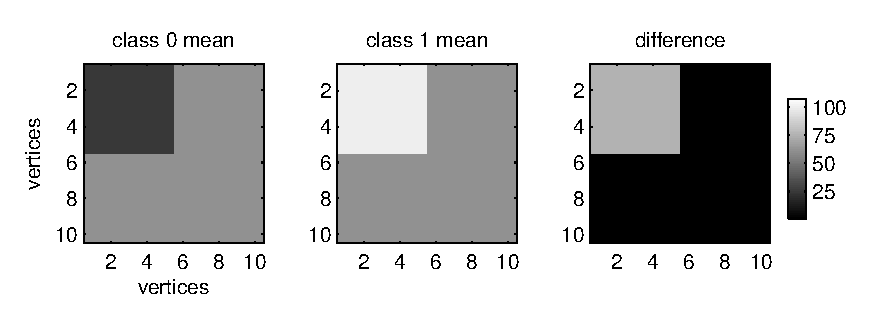
\includegraphics[width=0.5\linewidth]{../figs/homo_kidney_egg_model}
	\includegraphics[width=0.4\linewidth]{../figs/homo_kidney_egg_performance}
	\caption{Homogeneous-kidney-egg model simulation. The left and middle panels show the model parameters for class 0 and 1, respectively.  Each edge in the ``kidney'' in both classes has probability $0.5$; in the egg, class 0 edges are sampled with probability $0.25$, and class 1 edges are sampled with probability $0.75$. The right panel shows the QAP objective function (gray) and misclassification rate (black) as a function of iteration number. LAP does approximately as well as QAP on this (and other) simple graph simulation.  Note that $L_{chance}\approx 0.5$ and $L_* \approx 0$ for this simulation. The units of the right-side ordinate are arbitrary. The QAP objective function evaluation prior to any QAP iterations is beyond the bounds of this figure.}
	\label{fig:homo}
\end{figure}

% described above with $n_V=10$ vertices and $n=1000$ total samples, 500 from each class.  First, we generated a simulated homogeneous-kidney-egg problem, as depicted in Figure \ref{fig:homo_subfig1}.  Then, we run the Bayes Plugin \qapa algorithm described above.  Note that \qapa is an \emph{iterative} algorithm, so we can evaluate the performance of each iteration (not restart). 

% While Fig. \ref{fig:homo_subfig2} shows the QAP objective function decreasing with each iteration, Fig. \ref{fig:homo_subfig3} shows that classification performance does not decrease.  We found similar numerical results in two additional simulations: a heterogeneous-kidney-egg model (Figure \ref{fig:hke}) and a fully heterogeneous model (Figure \ref{fig:hetero}). Note that in all simulations $L_{chance} \geq \mh{L}_{QAP} \geq L_*$, as it must be.  Multiple iterations not improving classification performance led us to investigate the relationship between QAP and the Linear Assignment Problem (LAP).




\subsection{LAP vs. QAP} % (fold)
\label{sub:lap_vs_qap}

Much like the QAP objective function from Eq. \eqref{eq:QAP} can be simplified to Eq. \eqref{eq:qap}, the LAP objective function can be similarly simplified:
\begin{align}
	\argmin_{Q \in \mc{Q}} \norm{QA-B}_F^2 = \argmin_{Q \in \mc{Q}} tr(QA B\T).
\end{align}
Letting $f_{LAP}(Q)=tr(QA B\T)$, the gradient is:
\begin{align}
	% f_{QAP}(Q)	&= -tr(B\T QAQ\T) -tr(QAQ\T B)  &f_{LAP}(Q)&=-tr(AQ\T B\T) \\
	% \nabla_{QAP}&= AQB\T+A\T QB               	&
	\nabla_{LAP}&=2A B\T.
\end{align}
% Thus, when $Q=I$, the gradient of the QAP objective function is identical to that of the LAP objective function. Thus, one can use gradient ascent to to solve a LAP.  The gradient of $f'(Q)=\norm{AQ\T-B}_F^2$ is %:
% % \begin{align} \label{eq:grad2}
% 	$\partial f'/\partial Q = 2A B\T$. 
% % \end{align}
Comparing this gradient to that of QAP---Eq. \eqref{eq:grad}---one can see that when $Q^{(j)}$ is the identity matrix, the two gradients are identical.  Thus, if QAP is initialized at the identity matrix, the first permutation matrix---output of Step 2---is identical to $\mh{Q}_{LAP}$; although the line search will make $Q^{(1)} \neq \mh{Q}_{LAP}$, in general.  %Moreoever, projecting a matrix onto the closest permutation matrix can be written as a LAP because of the following relationship:
% \begin{align}
% 	\argmin_{Q \in \mc{Q}} \norm{QA\T - I}_F^2 &= \argmin_{Q \in \mc{Q}} (QA\T-I)\T (QA\T-I) 
% \nonumber\\ &=\argmin_{Q \in \mc{Q}} AQ\T QA\T -2QA\T - II = \argmin_{Q \in \mc{Q}}  -\langle Q, A\T \rangle  
% \end{align}
In the above simulation, the first iteration of \qap is essentially the only useful one.  Thus, we compare the performance of \texttt{BPI}$\circ$\texttt{LAP} (dark gray).  The performance of LAP and QAP are not statistically different for this simulation.  This suggests that for certain problems, LAP (which is $\mc{O}(n^3)$) is both an efficient and useful approximation to solving NP-hard graph matching problems. We were unable to find a model for simple graphs in which multiple iterations of \qap improved performance over LAP. %We confirm this intuition by substituting QAP with LAP in the above simulations (black line).  As depicted in the above figures, this intuition is consistent with the numerical results. In other words, while naively one might implement an algorithm with exponential time complexity, LAP, which is only quadratic time complexity, will often suffice.


% subsection lap_vs_qap (end)


\subsection{Multi-Graph simulation} % (fold)
\label{sub:heterogeneous_simulation}

Because \qapa works for both weighted and unweighted, we next simulated multi-graphs.  The below simulation is identical to the above except for $F_{uv|y}$---the edge random variable---was Bernoulli before and is now Poisson:  $F_{uv|y}=\text{Poisson}(a_{uv}; \lambda_{uv|y})$.  Figure \ref{fig:poiss} shows misclassification rate steadily decreasing with each iteration.

\begin{figure}[htbp]
	\centering			
	\includegraphics[width=0.5\linewidth]{../figs/poiss_model}
	\includegraphics[width=0.4\linewidth]{../figs/poiss_performance}
	\caption{Multigraph model simulation. The left and middle panels show the parameters for class 0 and  1, respectively.  The right panel shows the QAP objective function (gray) and misclassification rate (black) as a function of iteration number; both clearly descending.  For comparison, both $\mh{L}_{LAP}$ and $\mh{L}_*$ are shown.    }
	\label{fig:poiss}
\end{figure}

% subsection heterogeneous_simulation (end)


% \begin{figure}[ht]
% \centering
% \subfigure[model]{
% \includegraphics[scale=0.4]{../figs/hetero_kidney_egg_model}
% \label{fig:hke_subfig1}
% }
% \subfigure[objective function]{
% 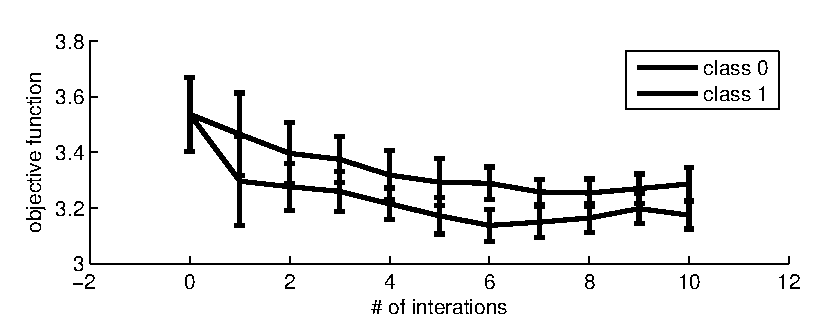
\includegraphics[scale=0.4]{../figs/hetero_kidney_egg_obj}
% \label{fig:hke_subfig2}
% }
% \subfigure[Lhat +/- Lstd]{
% \includegraphics[scale=1]{../figs/hetero_kidney_egg_Lhats}
% \label{fig:hke_subfig3}
% }
% \label{fig:hke}
% \caption{hetero kidney egg model}
% \end{figure}


\subsection{Connectome Classification} % (fold)
\label{sub:connectome_classification}

A ``connectome'' is a graph in which vertices correspond to biological neural units, and edges correspond to connections between the units.  Diffusion Magnetic Resonance (MR) Imaging and related technologies are making the acquisition of MR connectomes routine \cite{Hagmann2010}.  We use 49 subjects from the Baltimore Longitudinal Study on Aging, with acquisition and connectome inference details as reported in \cite{OHBM10}.  For each connectome, we obtain a $70 \times 70$ element adjacency matrix, where each element of the matrix encodes the number of streamlines between a pair of regions, ranging between 0 and about 65,000.  Associated with each graph is class label based on the gender of the individual (24 males, 25 females).  Because the vertices are labeled, we can compare the results of having the labels and not having the labels.  As such, we implement the following classification strategies.  In each case, we use a leave-one-out strategy to evaluate performance:

\begin{description}
	\item[\texttt{N/A-QAP}] Using the vertex labels, implement a standard $1$NN classifier, where distance is the norm of the difference between any pair of adjacency matrices.
	\item[\texttt{1-QAP}] Permute only the vertex labels of the test graph, and then implement \texttt{$1$NN$\circ$\qapa}.
	\item[\texttt{48-QAP}] Permuting the vertex labels, then implement \texttt{$1$NN$\circ$\qapa}.
	\item[\texttt{AVG-QAP}] Permuting the vertex labels, \qapa each of the 48 training graphs to the test graph.  Then, given those permuted adjacency matrices, compute the average, and then implement a standard $1$NN classifier.
	\item[\texttt{1NN-GI}] Use the graph invariant approach as described above. We provide the normalized graph invariants as inputs into a number of standard classifiers, including $k$NN, linear classifiers, support vector machines, random forests, and CW. On this data, the CW classifier performed best; we therefore only report its results.
\end{description}

Table \ref{tab:connectome} shows leave-one-out misclassification rates for the various strategies.


\begin{table}[h!]
\caption{MR Connectome Leave-One-Out Misclassification Rates}
\begin{center}
\begin{tabular}{|r|r|r|r|r|}
\hline
\texttt{N/A-QAP} & \texttt{1-QAP} & \texttt{48-QAP} & \texttt{AVG-QAP} & \texttt{1NN-GI}\\
\hline
$20\%$ & $31\%$ & $45\%$ & ?? & $25\%$ \\
    \hline
\end{tabular}
\end{center}
\label{tab:connectome}
\end{table}%


\section{Discussion}


In this work, we have presented a number of approaches one could take to classifier graphs.  Importantly, when the vertex labeling function is unavailable, one must deal with this uncertainty somehow.  We compare a number of approaches on both simulated and connectome data.  A multiple-restart Frank-Wolfe approach to approximating QAP outperforms previous state-of-the-art approaches in terms of approximating the graph matching problem.  Simulations demonstrate that only the first iteration of such an iterative algorithm, starting from the identity matrix, yields classification performance better than chance.  Moreover, the first iteration is identical to LAP, which is a linear problem with linear and non-negativity constraints, and therefore can be solved quite easily.  

On a connectome dataset, we compare the performance of various \qap classification algorithms with several graph invariant (GI) based strategies.  Of the algorithms that we tried, a graph invariant approach was most effective, even though, in theory, a QAP based approach could have done better (compare the first and last columns of Table \ref{tab:connectome}).  

These analyses leave many open questions.  Perhaps most interestingly, when might one expect a QAP-based approach to outperform a GI-based approach?  Resorting to a generative model, it should be clear that if the class conditional difference is independent of the vertex labels, then there is no reason to even try to implement graph matching.  However, if one believes that the labeling function might convey some class-conditional signal (as in the connectome data), then QAP-based approaches could outperform any approach that ignores the labeling function.  Which QAP-based approach to use in such a scenario, however, will depend on many factors, including the assumed model and computational resources.


% \subsubsection*{Acknowledgments}
% 
% Use unnumbered third level headings for the acknowledgments. All
% acknowledgments go at the end of the paper. Do not include 
% acknowledgments in the anonymized submission, only in the 
% final paper. 

% \subsubsection*{References}

\bibliography{/Users/jovo/Research/latex/library}
% \addcontentsline{toc}{section}{References}
\bibliographystyle{unsrt}
%\bibliographystyle{nature}

\end{document}
